\documentclass[14pt]{extbook}
\usepackage{multicol, enumerate, enumitem, hyperref, color, soul, setspace, parskip, fancyhdr} %General Packages
\usepackage{amssymb, amsthm, amsmath, bbm, latexsym, units, mathtools} %Math Packages
\everymath{\displaystyle} %All math in Display Style
% Packages with additional options
\usepackage[headsep=0.5cm,headheight=12pt, left=1 in,right= 1 in,top= 1 in,bottom= 1 in]{geometry}
\usepackage[usenames,dvipsnames]{xcolor}
\usepackage{dashrule}  % Package to use the command below to create lines between items
\newcommand{\litem}[1]{\item#1\hspace*{-1cm}\rule{\textwidth}{0.4pt}}
\pagestyle{fancy}
\lhead{Progress Quiz 4}
\chead{}
\rhead{Version A}
\lfoot{6286-1986}
\cfoot{}
\rfoot{Fall 2020}
\begin{document}

\begin{enumerate}
\litem{
First, find the equation of the line containing the two points below. Then, write the equation as $ y=mx+b $ and choose the intervals that contain $m$ and $b$.\[ (3, -4) \text{ and } (-9, -9) \]\begin{enumerate}[label=\Alph*.]
\item \( m \in [0.27, 1.6] \hspace*{3mm} b \in [-6.2, -4.1] \)
\item \( m \in [-0.58, 0.02] \hspace*{3mm} b \in [-12.9, -8.7] \)
\item \( m \in [0.27, 1.6] \hspace*{3mm} b \in [-7.7, -6.9] \)
\item \( m \in [0.27, 1.6] \hspace*{3mm} b \in [-0.9, 0.2] \)
\item \( m \in [0.27, 1.6] \hspace*{3mm} b \in [4.7, 5.7] \)

\end{enumerate} }
\litem{
Write the equation of the line in the graph below in Standard form $Ax+By=C$. Then, choose the intervals that contain $A, B, \text{ and } C$.
\begin{center}
    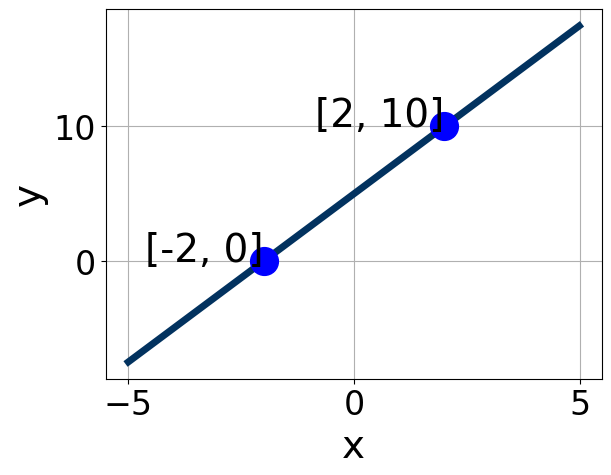
\includegraphics[width=0.5\textwidth]{../Figures/linearGraphToStandardCopyA.png}
\end{center}
\begin{enumerate}[label=\Alph*.]
\item \( A \in [-4, -1], \hspace{3mm} B \in [4.2, 5.9], \text{ and } \hspace{3mm} C \in [-28, -24] \)
\item \( A \in [-3.8, 3.2], \hspace{3mm} B \in [-1.8, 0], \text{ and } \hspace{3mm} C \in [1, 6] \)
\item \( A \in [1, 5], \hspace{3mm} B \in [-7.5, -3.6], \text{ and } \hspace{3mm} C \in [23, 26] \)
\item \( A \in [1, 5], \hspace{3mm} B \in [4.2, 5.9], \text{ and } \hspace{3mm} C \in [-28, -24] \)
\item \( A \in [-3.8, 3.2], \hspace{3mm} B \in [0.5, 4.4], \text{ and } \hspace{3mm} C \in [-12, -3] \)

\end{enumerate} }
\litem{
First, find the equation of the line containing the two points below. Then, write the equation as $ y=mx+b $ and choose the intervals that contain $m$ and $b$.\[ (6, 2) \text{ and } (-11, 10) \]\begin{enumerate}[label=\Alph*.]
\item \( m \in [-1.45, 0.23] \hspace*{3mm} b \in [-8.5, -4.7] \)
\item \( m \in [0.26, 0.51] \hspace*{3mm} b \in [13.4, 17.7] \)
\item \( m \in [-1.45, 0.23] \hspace*{3mm} b \in [-4.8, -0.2] \)
\item \( m \in [-1.45, 0.23] \hspace*{3mm} b \in [19.1, 22.9] \)
\item \( m \in [-1.45, 0.23] \hspace*{3mm} b \in [3.9, 5.3] \)

\end{enumerate} }
\litem{
Solve the equation below. Then, choose the interval that contains the solution.\[ -11(10x + 14) = -5(8x + 15) \]\begin{enumerate}[label=\Alph*.]
\item \( x \in [-3.31, -2.22] \)
\item \( x \in [-1.41, -0.84] \)
\item \( x \in [-1.55, -1.45] \)
\item \( x \in [2.49, 3.39] \)
\item \( \text{There are no real solutions.} \)

\end{enumerate} }
\litem{
Solve the equation below. Then, choose the interval that contains the solution.\[ -13(-19x + 17) = -9(-11x -18) \]\begin{enumerate}[label=\Alph*.]
\item \( x \in [-0.02, 0.19] \)
\item \( x \in [2.36, 2.61] \)
\item \( x \in [0.23, 0.59] \)
\item \( x \in [-0.59, -0.2] \)
\item \( \text{There are no real solutions.} \)

\end{enumerate} }
\litem{
Solve the linear equation below. Then, choose the interval that contains the solution.\[ \frac{-5x -3}{7} - \frac{3x + 6}{4} = \frac{-9x -3}{8} \]\begin{enumerate}[label=\Alph*.]
\item \( x \in [-18.68, -16.68] \)
\item \( x \in [-2.45, 3.55] \)
\item \( x \in [-5.58, -3.58] \)
\item \( x \in [2.26, 6.26] \)
\item \( \text{There are no real solutions.} \)

\end{enumerate} }
\litem{
Find the equation of the line described below. Write the linear equation as $ y=mx+b $ and choose the intervals that contain $m$ and $b$.\[ \text{Perpendicular to } 5 x + 6 y = 11 \text{ and passing through the point } (-5, -3). \]\begin{enumerate}[label=\Alph*.]
\item \( m \in [0.87, 1.62] \hspace*{3mm} b \in [1.5, 2.9] \)
\item \( m \in [0.59, 1.11] \hspace*{3mm} b \in [2.1, 3.8] \)
\item \( m \in [0.87, 1.62] \hspace*{3mm} b \in [2.1, 3.8] \)
\item \( m \in [-2.03, -0.73] \hspace*{3mm} b \in [-9.5, -8.2] \)
\item \( m \in [0.87, 1.62] \hspace*{3mm} b \in [-3.5, -0.6] \)

\end{enumerate} }
\litem{
Find the equation of the line described below. Write the linear equation as $ y=mx+b $ and choose the intervals that contain $m$ and $b$.\[ \text{Parallel to } 9 x + 8 y = 15 \text{ and passing through the point } (5, 4). \]\begin{enumerate}[label=\Alph*.]
\item \( m \in [-4, -1] \hspace*{3mm} b \in [-1.08, -0.21] \)
\item \( m \in [-1, 0.5] \hspace*{3mm} b \in [9.11, 10.01] \)
\item \( m \in [-0.5, 1.5] \hspace*{3mm} b \in [-2, -1.44] \)
\item \( m \in [-4, -1] \hspace*{3mm} b \in [-10.38, -9.31] \)
\item \( m \in [-4, -1] \hspace*{3mm} b \in [9.11, 10.01] \)

\end{enumerate} }
\litem{
Solve the linear equation below. Then, choose the interval that contains the solution.\[ \frac{-6x -3}{4} - \frac{-5x -7}{5} = \frac{4x -7}{6} \]\begin{enumerate}[label=\Alph*.]
\item \( x \in [8.61, 9.45] \)
\item \( x \in [0.47, 1.71] \)
\item \( x \in [-1.19, -0.43] \)
\item \( x \in [0.05, 0.55] \)
\item \( \text{There are no real solutions.} \)

\end{enumerate} }
\litem{
Write the equation of the line in the graph below in Standard form $Ax+By=C$. Then, choose the intervals that contain $A, B, \text{ and } C$.
\begin{center}
    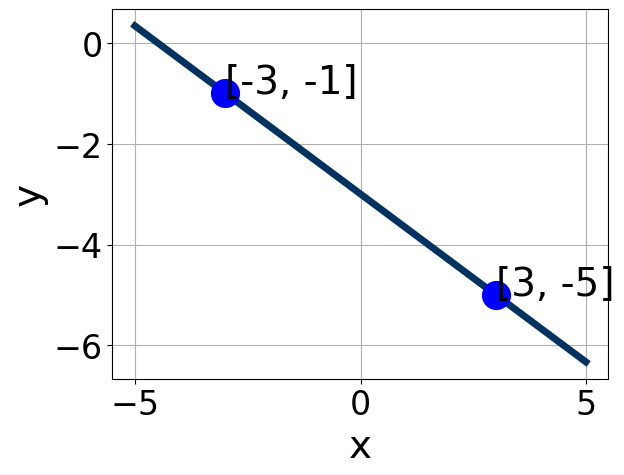
\includegraphics[width=0.5\textwidth]{../Figures/linearGraphToStandardA.png}
\end{center}
\begin{enumerate}[label=\Alph*.]
\item \( A \in [-0.1, 1], \hspace{3mm} B \in [-1.95, -0.91], \text{ and } \hspace{3mm} C \in [-5, 1] \)
\item \( A \in [1.6, 2.8], \hspace{3mm} B \in [1.98, 3.14], \text{ and } \hspace{3mm} C \in [4, 15] \)
\item \( A \in [-3, -1.8], \hspace{3mm} B \in [-3.03, -2.25], \text{ and } \hspace{3mm} C \in [-13, -6] \)
\item \( A \in [1.6, 2.8], \hspace{3mm} B \in [-3.03, -2.25], \text{ and } \hspace{3mm} C \in [-13, -6] \)
\item \( A \in [-0.1, 1], \hspace{3mm} B \in [-0.49, 2.74], \text{ and } \hspace{3mm} C \in [2, 8] \)

\end{enumerate} }
\end{enumerate}

\end{document}